\documentclass[../Main.tex]{subfiles}

\begin{document}
\chapter{Statistical Machine Learning}

\intro{

}

\section{Basics}
\defn{Correlation and Causation}{
\textbf{REMEMBER!} Correlation does not imply causation!
}
\subsection{Prediction vs Inference}
\defn{Statistical Machine Learning}{
    The main goal of statistical learning is to minimize the reducible error.
}
\defn{Error}{
    Output (dependable variable) depends not only on the input, but also a from \(X\) indepentend zero meanr error term \(\epsilon\). Even a perfect prediction function \(f(x_i)\) has a \textbf{irreducible error} \(\epsilon\).
\
    \begin{itemize}
        \item Random Measurement Error
        \item Systematic Errors e.g. humidity
    \end{itemize}

If the estimated \(\hat{f}(X)\) is not equal to the true function, there is the possibility to learn a better relationship between input and output, this is called \textbf{reducible error}.
\begin{equation}
    \begin{split}
        MSE&=E\{(Y-\hat{Y})^2\}\\
        &=(1)E\{(f(X)-\hat{f}(X))^2\}+(2)Var(\epsilon)\\
        (1)\text{Reducible Error }&+(2)\text{Irreducible Error}
    \end{split}
\end{equation}
    
}

\defn{Inference}{
    In inference we are interested in understanding the relationship between predictors and response. 
}

\defn{Estimation Aproaches}{
\begin{description}
    \item[Parametric] Assumptions are made about the functional form of \(f(X)\), where some missing parameters need to be learned. For example a simple linear model assumes form: \(f(X)=\beta_0+\beta_1X_1\).  If the form of \(\hat{f}(X)\) is far from \(f(X)\), then this approach achieves badly.
    \item[Non-Parametric]  Methods that make no assumptions about the functional form of \(f(X)\).
\end{description}
}

\defn{Supervised Learning}{
    In supervised learning for each input vector \(X\), its corresponding dependent variable \(Y\) is known.
}

\newpage
\section{Bias-Variance}
\begin{figure}[H]
    \centering
    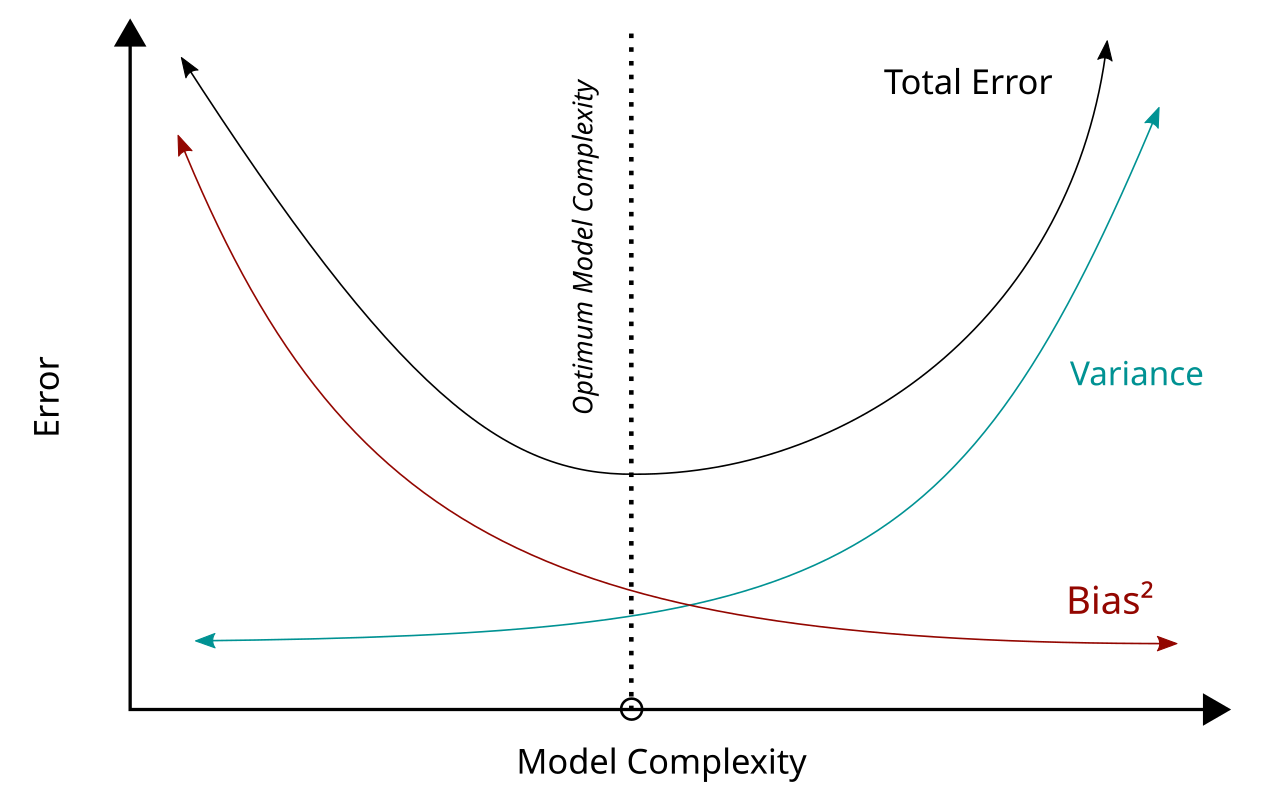
\includegraphics[width=0.75\linewidth]{Images/Bias_and_variance_contributing_to_total_error.svg.png}
    \caption{Bias Variance Tradeoff}
\end{figure}
The expected test MSE is the sum of a variance term, a bias term squared and the irreducible error.  Its defined as the average test MSE that would be obtained if \(f(X)\) is estimated repeatedly using a large number of training sets at tested at \(x_0\).
\begin{figure}[H]
    \centering
    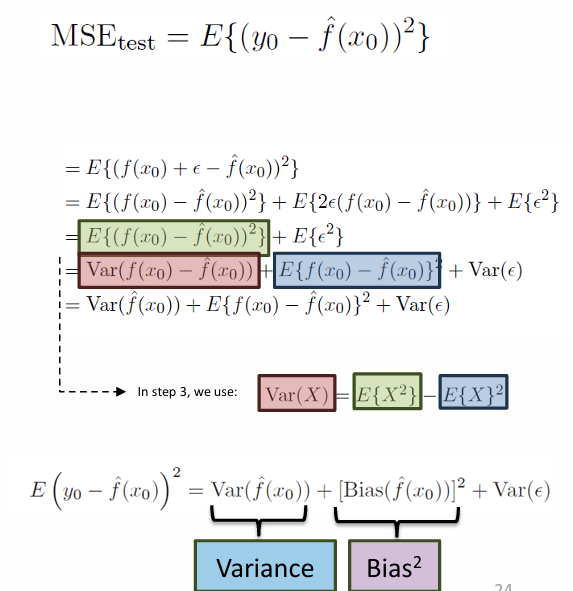
\includegraphics[width=0.5\linewidth]{Images/bias-variance-test-mse.png}
    \caption{Test MSE Equivalent}
\end{figure}
\newpage
The \(\sqrt{variance}\) refers to the amount by which the estimate would change, if we estimated using a different training set. Ideally the training set should have little influence on how the method estimates, this is typical for low flexibility methods.

The bias refers to the error introduces by approximating. If a model is too simple (low flexibility) to capture the true shape of the function, this will result in high bias.

\begin{figure}[H]
    \centering
    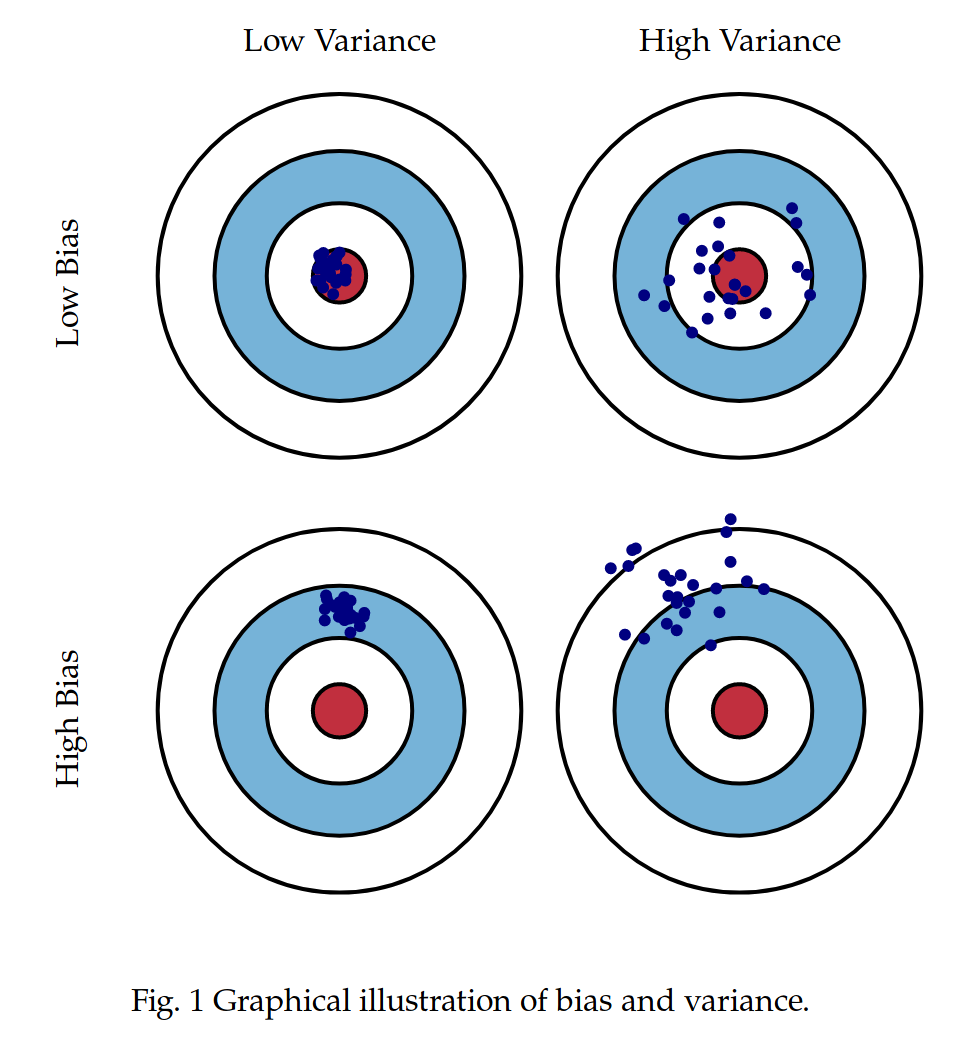
\includegraphics[width=0.5\linewidth]{Images/bias-variance-tradeoff.png}
    \caption{Bias Variance Tradeoff}
\end{figure}
\begin{figure}[H]
    \centering
    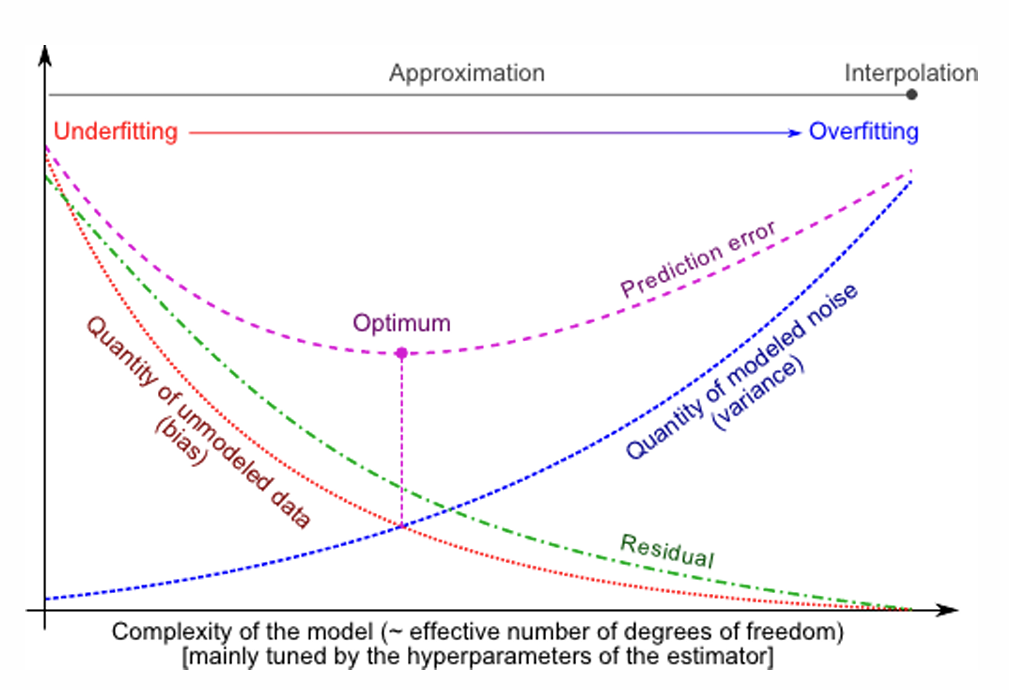
\includegraphics[width=0.5\linewidth]{Images/bias-variance-optimum.png}
    \caption{Bias Variance Tradeoff Optimum}
\end{figure}
\newpage
\defn{Bias-Variance Summary}{
 \begin{itemize}
     \item Flexible methods have low bias but high variance
     \item Simple methods have low variance but high bias

 \end{itemize}
}
\begin{figure}[H]
    \centering
    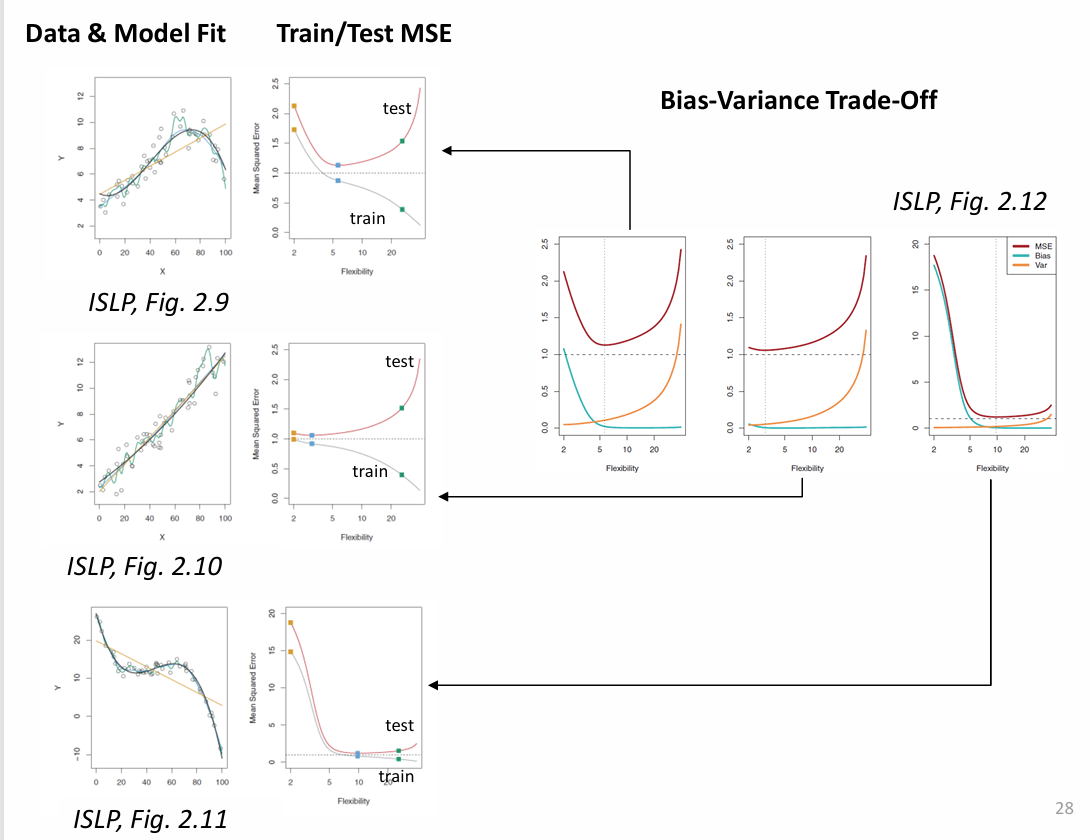
\includegraphics[width=1\linewidth]{Images/bias-variance-tradeoff-overview.png}
    \caption{Bias Variance Overview}
\end{figure}

\newpage
\section{Regression}
Quantitative (numerical) prediction where \(Y\) is an ordered numerical value. 
\defn{Mean Squared Error}{
\begin{equation}
    MSE = \frac{1}{N}(y_i-\hat{f}(x_i))^2
\end{equation}
}

\section{Classification}
Qualitative (categorical) prediction where \(Y\) is discrete categorical value. 
\defn{Classification Error Rate}{
\begin{equation}
    Error = \frac{1}{n}\sum_{i=1}^n I(y_i \ne \hat{y}_i)
\end{equation}
}

\defn{Bayes Classifier}{
    Test error rate is minimized, by a classifier that assigns each observation to the most probable class, given its predictor value. Results in the lowest possible error rate called Bayes error rate.
    \begin{equation}
        \begin{split}
            &Pr(Y=j|X =x_0)\\
            \text{set class to: }max_j(&Pr(Y=j|X=x_0))
        \end{split}
    \end{equation}
    Where \(j\) is the most probable class for a given input variable (predictor) \(X=x_0\). E.g for a 2 class model: \(Pr(Y=1|X=x_0)>0.5\)

    The bayes error rate is analogous to the irreducible error and is 0.1304.
}
\newpage
\defn{K-Nearest Neighbors}{
    Bayes classifier requires knowledge of the conditional distribution of \(Y|X\), in a real world problem this is never known. K-nearest neighbors is the simplest of such methods in which given a test point \(x_0\) KNN finds \(K\) neighbors and then estimates the class probabilities as the fraction of neighbors which belong to a particular class.

    \begin{equation}
        Pr(Y=j|X=x_0)=\frac{1}{K}\sum_{i\in N_0} I(y_i=j)
    \end{equation}
    Where \(N_0\) are the nearest neighbors to the point \(x_o)\).
    \begin{itemize}
        \item Small K results in high variance
        \item Big K results in high bias
        \item K controls the trade off
        \item \(\frac{1}{K}\) is a measurement of flexibility
    \end{itemize}
    
}
\begin{figure}[H]
    \centering
    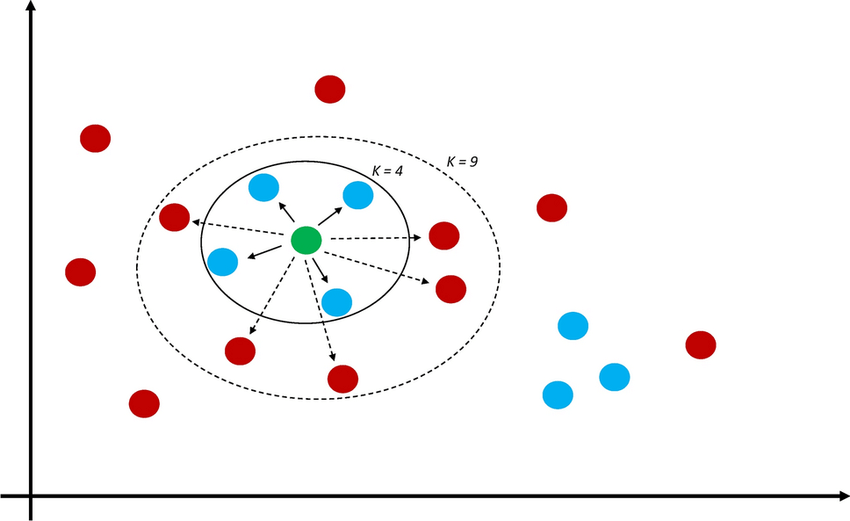
\includegraphics[width=0.75\linewidth]{Images/k-nearest.png}
    \caption{KNN}
\end{figure}

\begin{figure}[H]
    \centering
    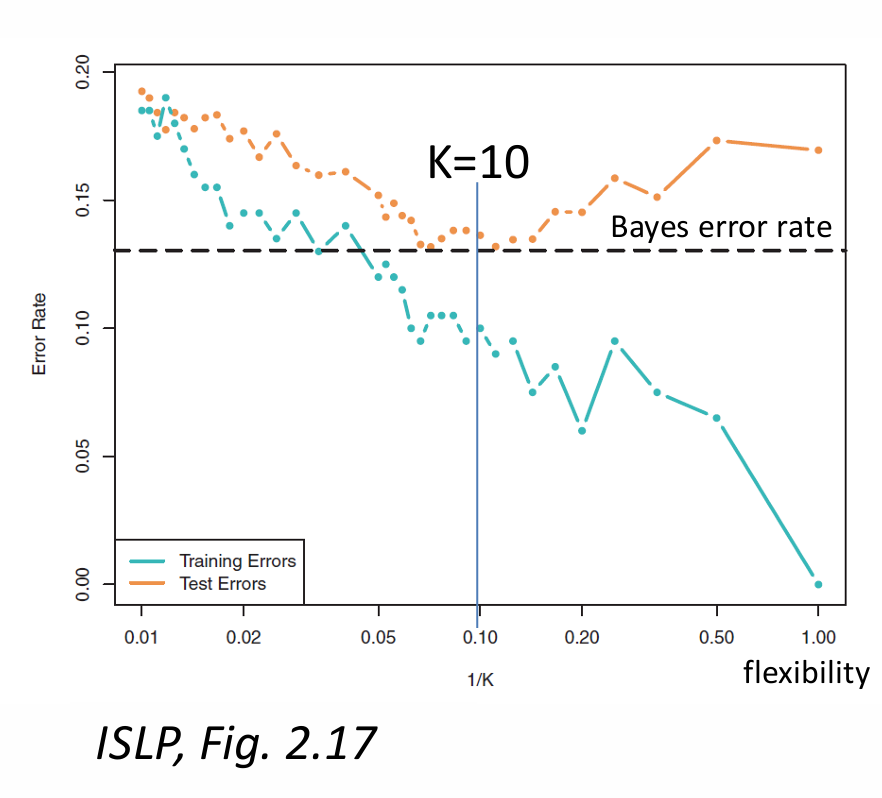
\includegraphics[width=0.5\linewidth]{Images/knn-flexibility.png}
    \caption{KNN Flexibility}
\end{figure}
\newpage
\section{Linear Regression}
\defn{Linear Regression Model}{
Estimates the linear relationship between a scalar response (dependent variable) and one or more explanatory variables (regressor or independent variable). There is a closed form solution for the RSS optimization.
\begin{equation}
    Y \approx \hat{Y} = \beta_0 + \sum_{i=0}^n \beta_{i+1} X_i
\end{equation}
By minimizing RSS:
\begin{equation}
    RSS = e_1^2+\dots+e_n^2 \text{ where } e_i = y_i-\hat{y}_i
\end{equation}

}
\subsection{Metrics}
\textbf{RSE} is roughly speaking, the average amount that the response will deviate from the true regression line. It provides an absolute measure of lack of fit of the model to the data. In fact the RSE carries the same unit as \(Y\).\textbf{ \(R^2\)} is the proportion of the variance explained by the model and hence it takes values between 0 and 1. \textbf{TSS} is the total sum of squares, which is the RSS if \(Y\) would always be predicted using the sample mean of \(Y\) (best possible predictor if we do not measure \(X\)). Assess accuracy of model with:
\defn{Model Accuracy}{
\begin{equation}
    \begin{split}
        RSE &= \sqrt{\frac{1}{n-p-1}RSS} \\
        TSS &= \sum (y_i - \bar{y} )^2 \\
         R^2 &= \frac{TSS-RSS}{TSS} = 1-\frac{RSS}{TSS} \\
    \end{split}
\end{equation}

}
\textbf{In simple linear regression} the following holds:
\begin{equation}
    R^2 = Cor(X,Y)^2 = Cor(Y,X)^2
\end{equation}
\textbf{In multivariate linear regression} the following holds:
\begin{equation}
    R^2 = Cor(Y,\hat{Y})^2
\end{equation}
We require a small variance of the estimate or equivalently a small standard error. Since \(\sigma^2\) is unknown it has to be estimated from data. Note that \(\sigma\) is the standard deviation of each independent realization of \(Y\).
\begin{equation}
    \begin{split}
         Var(\hat{\mu}) = SE(\hat{\mu})^2 = \frac{\sigma^2}{n}\\
         \text{where } \sigma^2 = Var(\epsilon)
    \end{split}
\end{equation}
Variance \(\sigma^2\) estimation using residual standard error (RSE):
\defn{Standard Error Estimation using RSE}{
    \begin{equation}
    \begin{split}
        \text{for }\sigma^2 &= Var(\epsilon) \\
        \implies SE\approx  \hat{SE} = RSE &= \sqrt{\frac{RSS}{n-n_\beta}}
    \end{split}
\end{equation}
}
Under the Gaussian assumption confidence intervals can be computed using the estimated variance. 
\defn{Confidence Intervals}{
    \begin{equation}
    Pr(a<\hat{b}_i<b)=0.95 \implies \hat{\beta}_i \pm 2\cdot \hat{SE}(\hat{\beta}_i)
\end{equation}
}
\subsection{T-Test}
The T-test (with the T-statistic), is a tool for evaluating the means of one or two populations using hypothesis testing) Hypothesis tests using null hypothesis. We can test the relevance of coefficients using the T-test:
\defn{T-Test for Coefficients}{

\begin{equation}
    \begin{split}
        H_0 : \text{There is no relation between }X \text{ and }\\
        \text{or } b_i = 0 \\
        H_a : \text{There is a relationship}
    \end{split}
\end{equation}
\begin{equation}
    \text{T-statistic} = \frac{\hat{\beta}_i}{\hat{SE}(\hat{\beta}_i)}
\end{equation}
With \(n-n_\beta\) degrees of freedom where p:
\begin{equation}
    p = Pr(|T|>|t| \qquad | H_0)
\end{equation}
}
\textbf{P-Value} is the probability that we realistically observe an absolute T-value equal or bigger to the one observed under the \(H_0\).

\subsection{F-Test}
An F-test is any statistical test used to compare the variances of two samples or the ratio of variances between multiple samples. To check if there is any relationship between predictors and the dependent variable the F-test can be used:
\defn{F-Test}{
    \begin{equation}
    \begin{split}
        H_0 &: \beta_0 = \dots = \beta_n = 0 \\
        H_a &: \text{at least one } \beta_j \text{ is non-zero} \\
        \text{using F-statistic} &: F=\frac{(TSS-RSS)/p}{RSS(n-p-1)}\\
        \text{and} &: TSS = \sum (Y_i-\bar{y})^2 \text{, } RSS=\sum (y_i - \hat{y})^2
    \end{split}
\end{equation}
}
F-statistic expresses the improvement of the model per parameter \(p\) in multiples of the residual variance. If the linear model assumptions are correct and \(H_a\) is true we expect the F-statistic on average to be greater than one.

One can also use a subset of \(q\) coefficients to test with a new hypothesis. We order the predictor variables so that the last q variables are the one to test for being zero. Then we fit a second model that uses all the predictor variables except the last q .
\begin{equation}
    F = \frac{(RSS_0-RSS)/q}{RSS/(n-p-1)}
\end{equation}
\defn{Single Coefficient F-Test}{
    When we leave out only one variable (q=1) then the F-statistic would tell the partial effect of adding that variable to the model. \textbf{It turns out, the F-statistic, if only one variable is left out, is identical to the squared T-statistic.}
}

\subsection{Predictor Selection}
\begin{itemize}
    \item Forward selection
    \item Backward selection
    \begin{itemize}
        \item Cannot be used if there are more predictor variables than training samples
    \end{itemize}
    \item Mixed Selection
\end{itemize}

\section{TODO: ADVANCED LINEAR REGRESSION TOPICS}

\section{Unsuperviced Learning}
In UL there is no response variable \(Y\), only
predictors \(x_1,\dots ,x_n\). These are measured in
\(n\) observations resulting in the data matrix \(X\)
of dimension \(nxp\). The goal is to gather
inference data using methods like dimensionality reduction
and clustering. The methods require human judgement and have
thus a subjective nature.
\subsection{Principal Component Analysis}
You have your dataset \(X\) up to \(X_p\) with \(n\) rows.
Now you reduce it to include fewer features by incorporating
information into less variables. In PCA regression the idea
was to reduce the dimensions and then to apply a regression model.
This will lead to lower flexibility and thus lower variance.

Without regression we skip the training of a prediction model.
The method stays the same. We try to fit a line to our data
that contains the largest variance.

\defn{PCA}{
    Find a linear transform for principal component for which
    a set of features is a normalized linear combination
    of the features, resulting in the largest variance:
    \begin{equation}
        \begin{split}
            Z_1 &= \Phi_{11} X_1 + \Phi_{21}X_2+\dots+\phi_{p1}X_p \\
            \text{For which: } Z_1 = &max(var(Z_1))
        \end{split}
    \end{equation}
    \(Z_1\) denotes the first principal component. We choose
    a linear mapping to keep a simple representation.
    One could also choose a non linear transformation (T-SNE).

    With the loading vector of \(Z_1\):
    \begin{equation}
        \Phi_1 = (\Phi_{11},\dots,\Phi_{p1})^T
    \end{equation}
    Each entry \(\Phi\) is called loadings of \(Z\).
    The sum of the loadings squared and summed up must equal to 1:
    \begin{equation}
        \sum_{j=1}^{p} \Phi_{j1}^2=1
    \end{equation}
    In other words the loadings vector must have norm or length of one.
    Otherwise, the variance can be made arbitrarily large, by selecting
    large loadings.

    Before applying PCA the first step would be to normalize the data
    matrix \(X\). This is done by centering the columns (predictor variables)
    to have zero mean, by subtracting the sample mean of each column from
    the respective column. Often also division by sample SE.

}

\subsubsection{Scatter-Plot}
PCA is very useful for data visualisation. For example, we
can use PCA to reduce dimension in order to create a scatter plot.
Without PCA the amount of plots would equate to:
\begin{equation}
    \binom{p}{2} = \frac{p(p-1)}{2}
\end{equation}



\subsection{Clustering}

\end{document}